\documentclass{article}
\usepackage{amsmath}
\usepackage{xcolor}
\usepackage{gensymb}
\usepackage{ragged2e}
\usepackage{graphicx}
\usepackage{gensymb}
\usepackage{mathtools}
\newcommand{\mydet}[1]{\ensuremath{\begin{vmatrix}#1\end{vmatrix}}}
\providecommand{\brak}[1]{\ensuremath{\left(#1\right)}}
\providecommand{\norm}[1]{\left\lVert#1\right\rVert}
\newcommand{\solution}{\noindent \textbf{Solution: }}
\newcommand{\myvec}[1]{\ensuremath{\begin{pmatrix}#1\end{pmatrix}}}
\let\vec\mathbf
\begin{document}
\begin{center}
        \textbf\large{CHAPTER-7 \\ TRIANGLES}
\end{center}
\section{Exercise 7.1}
Q1. In quadrilateral $CBAD$,$CA = AD$ and $BA$ bisect $\angle{A}$ shown in figure \ref{fig:Fig1}. Show that $\triangle{CAB} \cong \triangle{DAB}$. What can you say about $BC$ and $BD$? \\
\textbf{Construction}\\
\begin{figure}[h]
	\begin{center}
		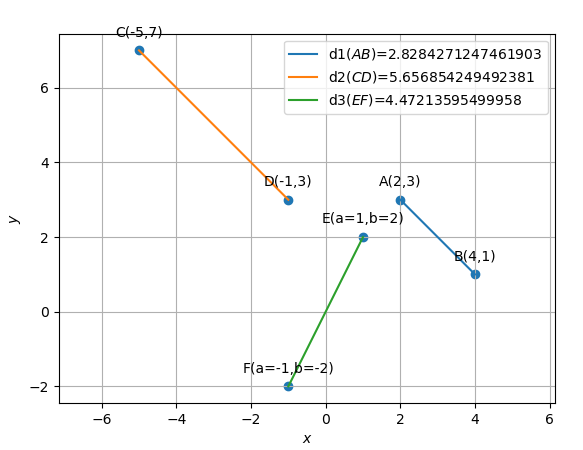
\includegraphics[width=\columnwidth]{figs/graph.png}
	\end{center}
	\caption{Quadrilateral CBAD}
	\label{fig:Fig1}
\end{figure}
\pagebreak
\\ The input parameters for construction are shown in \ref{tab:Table1}:\\
\begin{table}[h]
	  \centering
	  \begin{tabular}{|p{3cm}|p{3cm}|p{3cm}|}
\hline                                        
\textbf{Symbol} & \textbf{Values} & \textbf{Description}\\                                          
\hline                                 
$\theta$ & 30$\degree{}$   & $\angle{BAD} = \angle{BAC}$ \\           
\hline                                    
a &  9 & $AB$ \\     
\hline                      
c & 5 & $AC$ \\
\hline                                     
		$\vec{e}_1$ & $\myvec{
			1\\
			0\\
			}$ & basis vector\\ 
\hline
\end{tabular}

	  \caption{Parameters}
	  \label{tab:Table1}
\end{table}
\begin{align}
	\vec{A} = \myvec{0\\0},\vec{B} = a\vec{e_1},\vec{C} = \myvec{c\cos\theta\\c\sin\theta},\vec{D} = \myvec{c\cos\theta\\-c\sin\theta}
\end{align}
\solution
\begin{align}
	\vec{C}-\vec{A} &= \vec{A}-\vec{D}\\
	\angle{CAB} &= \angle{DAB}
\end{align}
\textbf{To Prove:}
	\begin{align}
		\triangle{CAB} \cong \triangle{DAB}
	\end{align}
\textbf{Proof:}\\
In $\triangle{CAB}$ and $\triangle{CAD}$\\
Let  equation of $AB$ be $y = 0$, which can be written as:
\begin{align}
	\vec{n}^{\top}\vec{x} = 0,\\
\end{align}
where
\begin{align}
\vec{x} = \myvec{x\\y},\vec{n} = \myvec{0\\1}
\end{align}
	Finding the angles(according to assumptions):
		\begin{align}
\text{Let }\theta_1=&\angle CBA\\
\vec{m_1}=&\vec{B}-\vec{C}=\myvec{4.7\\-2.5}, \vec{m_2}=\vec{B}-\vec{A}=\myvec{9\\0}\\
\theta_1=&\cos^{-1}\frac{\vec{m_1}^\top\vec{m_2}}{\norm{\vec{m_1}}\norm{\vec{m_2}}}\\
\implies\theta_1=&\cos^{-1}\frac{\myvec{4.7&-2.5}\myvec{9\\0}}{(9.2)(9)}=59.3\degree
\label{eq:1}\\
\text{Let }\theta_2=&\angle ABD\\
\vec{n_1}=&\vec{D}-\vec{B}=\myvec{-4.7\\2.5}, \vec{n_2}=\vec{A}-\vec{B}=\myvec{-9\\0}\\
\theta_2 =& \cos^{-1}\frac{\vec{n_1}^\top\vec{n_2}}{\norm{\vec{n_1}}\norm{\vec{n_2}}}\\
\implies\theta_2=&\cos^{-1}\frac{\myvec{-4.7&2.5}\myvec{-9\\0}}{(9.2)(9)}=59.3\degree
\label{eq:2}\\
\end{align}
from $\eqref{eq:1}$ and $\eqref{eq:2}$
\begin{center}
$\angle$ BAC = $\angle$ BAD \text{ (Sum of the angles in a triangle = 180\degree) }
\end{center}
Since all the angles and sides of triangles $CAB$ and $CAD$ are equal , from the definition of congruency both the triangles are said to be congruent to each other.
\begin{align}
	\triangle{CAB} &\cong \triangle{DAB}\\
	AB &= AD 
\end{align}
\end{document} 
